%-----------------------------------------------------------------------------
%
%               Template for sigplanconf LaTeX Class
%
% Name:         sigplanconf-template.tex
%
% Purpose:      A template for sigplanconf.cls, which is a LaTeX 2e class
%               file for SIGPLAN conference proceedings.
%
% Guide:        Refer to "Author's Guide to the ACM SIGPLAN Class,"
%               sigplanconf-guide.pdf
%
% Author:       Paul C. Anagnostopoulos
%               Windfall Software
%               978 371-2316
%               paul@windfall.com
%
% Created:      15 February 2005
%
%-----------------------------------------------------------------------------


\documentclass[10pt,numbers]{sigplanconf}
\usepackage[1stsubmission]{oopsla2016}

% The following \documentclass options may be useful:

% preprint      Remove this option only once the paper is in final form.
% 10pt          To set in 10-point type instead of 9-point.
% 11pt          To set in 11-point type instead of 9-point.
% numbers       To obtain numeric citation style instead of author/year.

\usepackage{amsmath}
\usepackage{graphicx}
\usepackage{listings}
\usepackage{xcolor}
\usepackage{amsmath}
\usepackage{semantic}
\usepackage{url}
\usepackage{natbib}
\bibliographystyle{plainnat}
\usepackage[utf8]{inputenc}
\usepackage[english]{babel}
\usepackage{stmaryrd}
\usepackage{pgf}
\usepackage{caption}
\usepackage{subcaption}
\usepackage{wasysym}
\usepackage{tikz}
\usetikzlibrary{arrows,automata}

\lstset{
         language=Java,
         basicstyle=\scriptsize\ttfamily, % Standardschrift
         %numbers=left,               % Ort der Zeilennummern
         numberstyle=\tiny,          % Stil der Zeilennummern
         %stepnumber=2,               % Abstand zwischen den Zeilennummern
         numbersep=5pt,              % Abstand der Nummern zum Text
         tabsize=1,                  % Groesse von Tabs
         extendedchars=true,         %
         breaklines=true,            % Zeilen werden Umgebrochen
         keywordstyle=\bf, %\underline,
         morekeywords={find,in,when,then,let,not,letrec,act,self,become,export,probably,and},
         %numbers=left,
         escapeinside={(*}{*)},
         moredelim=[is][\color{blue}\underbar]{@}{@},
         moredelim=[is][\bf\underbar]{^}{^},
         literate={fun}{$\lambda$}{1}{->}{$\rightarrow$}{1}{<-}{$\leftarrow$}{1}{...}{$\ldots$}{1}{insymb}{$\in$}{1}{nothing}{$\epsilon$}{1}{box}{$\boxempty$}{1}{mu}{$\mu$}{1}{circ}{$\ocircle$}{1},
         %deletekeywords={new},
         showspaces=false,           % Leerzeichen anzeigen ?
         keepspaces=true,
         showtabs=false,             % Tabs anzeigen ? 
         showstringspaces=false      % Leerzeichen in Strings anzeigen ?        
 }
 
 \def\code#1{{\normalfont\lstinline[basicstyle=\small\ttfamily]{#1}}}
\def\bar{\mathop{|}}
\newcommand{\cL}{{\cal L}}

\begin{document}

\special{papersize=8.5in,11in}
\setlength{\pdfpageheight}{\paperheight}
\setlength{\pdfpagewidth}{\paperwidth}

\conferenceinfo{CONF 'yy}{Month d--d, 20yy, City, ST, Country}
\copyrightyear{20yy}
\copyrightdata{978-1-nnnn-nnnn-n/yy/mm}
\copyrightdoi{nnnnnnn.nnnnnnn}

% Uncomment the publication rights you want to use.
%\publicationrights{transferred}
%\publicationrights{licensed}     % this is the default
%\publicationrights{author-pays}

%\titlebanner{banner above paper title}        % These are ignored unless
%\preprintfooter{short description of paper}   % 'preprint' option specified.

\title{ESL: An Enterprise Simulation Language}
%\subtitle{Subtitle Text, if any}

%\authorinfo{Tony Clark}
%           {Sheffield Hallam University, UK}
%           {t.clark@shu.ac.uk}
%\authorinfo{Vinay Kulkarni, Souvik Barat}
%           {Tata Consultancy Services Research, India}
%           {vinay.vkulkarni@tcs.com, souvik.barat@tcs.com}
%\authorinfo{Balbir Barn}
%           {Middlesex University, UK}
%           {b.barn@mdx.ac.uk}

\authorinfo{Author}{Affiliation}{email}

\maketitle

\begin{abstract}
Computational support for organisational decision-making is an emerging field where challenges arise from characteristic features such as complexity, emergent socio-technical behaviour, collaborative behaviour, and dependencies between objectives. Current approaches are mostly either human-centric or are based on technologies such as spreadsheets and equational models such as {\it stock and flow}. A number of researchers have proposed using {\it agents} to model aspects of organisations and thereby support decision-making, but there is no widely accepted approach. This paper develops existing work in this area by proposing a conceptual model for organisational decision-making and introduces an actor-based language called ESL for simulation of the concepts. The approach is demonstrated via a the implementation of a synthetic example and evaluated using a real-world example from industry.
\end{abstract}

\category{I.6.2}{Simulation Languages}{}

\keywords
enterprise modelling, multi-agent simulation.

\section{Introduction}

Organisational decision-making is a hard problem and we have few tools to help understand and address the area. The existing tools do not adequately represent the characteristic features of the problem and this has led to a proposal for using agent-based approaches as described in section \ref{sec:related_work}. 

Agents seem to offer a better basis for the characteristic features of an organisation, however there is no conceptualisation of agent-based systems that is appropriate for decision-making; section \ref{sec:concepts} analyses the problem domain and presents such a conceptual model that has been used by the authors as the basis of real-word case studies including that described in this paper.

We lack appropriate models for organisational decision-making that can help motivate the development of supporting technologies. Given that the problem domain is large and variegated, it makes sense to divide and conquer by seeking specific scenarios. A typical example relates to how commercial advantage can be achieved within a market that is created when multiple customers offer up opportunities for competitive bid by service providors. A framework for modelling this situation is described in section \ref{sec:bidding}. 

Our proposed approach is to view such a situation through the lens of the conceptual model and then to represent the resulting concepts in a technology that is suitable for simulation. In order to achieve this we require an appropriately expressive technology that supports translation of the problem domain concepts into agent-based solution domain patterns. We have found that the Actor Model of computation provides a suitable metaphor for such an encoding and have designed a language called ESL to support this approach whose  implementation is described in section \ref{sec:ESL}.

The contribution of this work is to propose a conceptual model for agent-based simulation of organisations and to provide a language for a suitable computational implementation platform. These contributions are provided in sections \ref{sec:concepts} and \ref{sec:ESL} and demonstrated in terms of a synthetic framework for bidding in section \ref{sec:simulation}. Evaluation of the approach is provided by a real-world case study taken from the software services domain operating within Tata Consultancy Services as described in section \ref{sec:evaluation}.

\section{Related Work}

\label{sec:related_work}

Enterprise Modelling (EM) \cite{vernadat2002ueml} aims to reduce dependence on human experts for organisational decision making. However, the languages capable of modelling all relevant aspects, {\it e.g.}, the aspects suggested by Zachman in \cite{zachman1987framework}, lack support for automated analysis. In contrast, languages providing automated support for qualitative and/or quantitative analyses are capable of modelling only one aspect of enterprise \cite{barjis2010relevance}. Therefore, a decision maker is forced to construct a tool-chain involving a large spectrum of EM tools \cite{camus2015combining} which is a challenging task.

The general industry practice is to follow a refinement-based method, {\it e.g.}, \cite{mintzberg1976structure}, for organizational decision making that is guided by separation of concerns driven by goal analysis, their dependencies, the means of achieving the goals and their qualitative and quantitative differences. Such analysis raises questions relating to the {\it levers} and {\it measures} that are used to undertake decision-making and ultimately differentiate between alternatives \cite{cyert1963behavioral,mintzberg1976structure}.

Languages such as Archimate \cite{iacobstate}, EEML \cite{krogstie2008using} and IEM \cite{bernus2013handbook} enable the specification of multiple aspects in an integrated manner. Archimate visualizes an enterprise along three aspects: {\it structural}, {\it behavioural} and {\it information}, and three levels: {\it business}, {\it application} and {\it technology}. IEM visualises an enterprise along two aspects: {\it information} and {\it process}. These structured representations help to improve documentation quality but lack precise analytical semantics necessary for decision-making. As a result, these frameworks are vulnerable to multiple interpretations and rely heavily on human analysis.

Modelling languages such as BPMN \cite{white2004business}, i* \cite{yu2006exploring} and stock-n-flow (SnF) \cite{meadows2008thinking} are machine processable but support modelling of one aspect only. For example, the process aspect can be modelled using BPMN, high level goals and objectives can be modelled using i*, and high level dynamics can be modelled using SnF. Amongst these machine processable languages, i* supports only qualitative analysis whereas BPMN and SnF support only quantitative analysis. 

There are language-specific peculiarities and limitations too: SnF modelling tools such as iThink\footnote{\url{iseesystems.com/Softwares/Business/ithinkSoftware.aspx}} and Simantics\footnote{\url{sysdyn.simantics.org/}} come with a rich simulation machinery supporting what-if simulation, however, the language is best suited for creating generic models which explode in size when specialised; several BPMN tools such as ARIS\footnote{\url{ariscommunity.com/university/downloads/aris-business-architect}} and Bizagi\footnote{\url{www.bizagi.com/}} support what-if simulation but only in terms of time and behavioural resource parameters. Moreover, the three languages being paradigmatically diverse, it is difficult to integrate individual specifications in a meaningful manner \cite{chen2008architectures,fox1993issues,barjis2008enterprise}, for example, the support available for specifying relationships across these aspects in AnyLogic\footnote{\url{anylogic.com/}} is little more than setting up navigation links from one specification to the other.

There is limited reported work on integration of multiple languages where each language supprts a different aspect of an organisation. The Unified Enterprise Modelling Language (UEML) \cite{vernadat2002ueml} initiative aims to integrate existing Enterprise Modelling Languages using a meta-modelling framework. This is an ongoing initiative \cite{opdahl2007roadmap} with the first version of the UEML demonstrating integration of IEM, EEML and GRAI \cite{doumeingts1993gim} supported by MOOGO\footnote{\url{moogo.de}} and METIS\footnote{\url{enterprise-architecture.info/Images/Computas Metis/Metis overview.htm}}.

We aim to support decision-making by taking a {\it computational approach} to organisational modelling \cite{weinhardt2012computational}. This builds on existing approaches described above that identify the key conceptual features and previous work by the authors 
(citations suppressed).
%\cite{DBLP:journals/emisaij/ClarkB13,DBLP:conf/caise/KulkarniBCB15,DBLP:conf/models/KulkarniBCB15}. 
We believe that the Actor Model of computation \cite{hewitt2010actor} is a suitable basis because it can support adaptive and emergent behaviour suitable for socio-technical systems \cite{gill2015adaptive,beese2015conceptualization}. Our aim is that the actor model can be used to develop a multi-agent systems based approach to organisational simulation and decision-making \cite{lee2015complexities,tan2013framework,camarinha2001virtual}.

There are several languages that use the actor model of computation \cite{ricci2015special} many of which address the issue of easing the engineering challenge of developing concurrent software. Our motivation is slightly different: to provide an expressive basis for organisational simulation. ESL has the notion of time built-in to its executive since this seems to be key to co-ordination of units within a simulation.

\section{Conceptual Model}

\label{sec:concepts}

A variety of Enterprise Modeling (EM) languages exist that provide information-capture and analysis support. The majority of these languages can be traced to the Zachman framework that is defined in terms of {\it why}, {\it what}, {\it how}, {\it who}, {\it when} and {\it where}. Many languages ({\it e.g.}, Archimate) provide a rich collection of modelling concepts for these concepts, however previous work (citations suppressed) has proposed that for the purposes of computational simulation and analysis the features can be reduced to a much smaller set of concepts.

Our aim is to view an organisation as a socio-technical system where the intrinsic complex emergent behaviour is achieved by representing parts of the organisation as goal-driven autonomous self-aware adaptive units. This section describes the conceptual model that underpins the approach and that is implemented using the language ESL later in the paper.

\begin{figure}[t]
\includegraphics[width=\columnwidth]{unit}
\caption{Conceptual Model}
\label{fig:conceptual_model}
\end{figure}

Figure \ref{fig:conceptual_model} shows the proposed conceptual model. An organisation is represented as a collection of units. A unit is used to represent anything that can act or be acted upon within an organisation and may correspond to a person, a resource, a department, a self-organised collection of individuals, {\it etc}. Units have internal state which can change over time giving rise to a history of states. Units may be composite and therefore have children, for example a department contains employees. Units may reference each other and there is an expectation that there is some notion of control whereby contained information can be designated {\it public} or {\it private}.

A unit is autonomous and therefore has behaviour that acts on the unit's state. Unit interaction is message-based with the assumption that messages can be both synchronous and asynchronous.

Units have a goal that drives their behaviour. This is an important feature of many aspects of an organisation viewed as a socio-technical system. A goal is a predicate over the history of a unit and it is therefore possible to determine at any given time whether a unit is satisfying its goal. A unit is free to dynamically change its goal, and, since units may be composite, a goal may relate to multiple units.

Units are self-adaptive, meaning that they can influence their behaviour through introspection. The conceptual model associates a unit with an adaptor that monitors the unit's goal. If the adaptor detects that the unit is not on target to achieve its goal then adaptation occurs via self-directed messages.
%
Simulation is supported by augmenting figure \ref{fig:conceptual_model} with:
\begin{description}
\item[measures]
A simulation is performed in order to support decision-making in terms of goals, for example: whether a goal is achieved, or the comparison of different configurations with respect to the same goal, or whether one goal is in some way more attractive than another. A goal is a predicate over unit histories and therefore a simulation measure can be conceptualised as a goal.
\item[levers]
 Multiple simulations are performed in order to compare different configurations of an organisation. Differences may include: unit configurations, behavioural traits, or adaptation. Levers are a conceptualisation of variations and generalise figure \ref{fig:conceptual_model} in the sense of Software Product Lines \cite{DBLP:books/daglib/0032299}.
\end{description}

\section{Decision Making: Competitive Bidding}

\label{sec:bidding}

\begin{figure}[t]
\includegraphics[width=\columnwidth]{service_providers}
\caption{Competitive Bidding}
\label{fig:competitive_bidding}
\end{figure}

Commercial organisations often participate in a market for products and services. Customers have requirements for the products that they make available as an {\it invitation to tender}. Providers are given a period of time within which they can produce a description of how they meet the requirements and what the cost will be. At the end of the bidding period, a customer evaluates  bids using their private criteria. One of the providers (the {\it winner}) is chosen and all other providers lose the bid.

Figure \ref{fig:competitive_bidding} shows a diagram containing customers, providers and a global notice-board that contains the public invitations to tender. In this simple scenario, each customer represents their internal requirements as a colour: either red or green. When the tender is made public on the notice-board, the providers do not know the private colour that the customer requires. Each provider chooses to bid red or green. After a period of time the customer inspects the bids and chooses one that matches their required colour. Each provider is shown with a history of bid-successes and bid-failures.

Although each provider does not know the required colour of the published tender, they can inspect the history of each customer in terms of their required colours over time. It is reasonable to expect that a customer repeatedly issues invitations of a particular colour and that there is a small probability that this colour will change at any time.

In such a situation we may take the role of a provider and aim to determine a strategy that will improve our chance of winning a bid. In this case the strategic options are the levers: (1) simply take a random chance; (2) stick with the same colour over time; (3) try to observe the behaviour of one or more customers via their history and predict the next requirement. Given that competitors may be using similar strategies, it is attractive to use a simulation-based approach to measure the outcomes for each option.

The situation shown in figure \ref{fig:competitive_bidding} is clearly very simple, but it establishes a basic framework within which competitive bidding can be investigated through the use of simulation. This paper will show how the framework, as described, can be modelled and simulated. 

Figure \ref{fig:conceptual_model} shows the conceptual model for our approach. The competitive bidding example can be viewed in terms of these concepts as follows. Customers, providers, notice-boards and opportunities to tender are units. All units respond to messages from a global clock that drives the simulation. Customers use the time messages to schedule opportunities. Providers use the time messages to regularly inspect the notice-board for opportunities. An opportunity uses time messages to award itself to a provider whose offering matches a requirement and to inform the customer of the outcome. The histories of the units are as shown in figure \ref{fig:competitive_bidding} and the goal of a provider is to win as many opportunities as possible.

In the simple case we may be using the simulation from the perspective of a distinguished provider {\it p} in order to determine a bidding strategy. Therefore the simulation measure is the number of wins by {\it p} and the levers of the simulation vary the provider's adapter in order to maximise the number of wins.

We believe that the framework can form the basis of a wide range of variations and increasingly sophisticated models. For example, the customer requirements are given as red or green, however in a real-world situation the requirements will have a range of properties that govern whether the bid from a provider is acceptable compared to that of another provider. The information available to a provider in terms of the behavioural history of a customer and of its competitors can be made more detailed. Other aspects such as negotiation and collaboration can be introduced allowing, for example, multiple providers to work together in order to maximise the chance of collectively winning a bid.

\section{ESL: An Enterprise Simulation Language}

\label{sec:ESL}

\begin{figure}
\begin{lstlisting}
exp  ::= var                         variables
     |   num                         numbers
     |   bool                        booleans
     |   str                         strings
     |   self                        active actor
     |   null                        undefined
     |   new name (exp*)             create actor
     |   become name (exp*)          change behaviour
     |   exp op exp                  binary exp
     |   not exp                     negation
     |   fun(name*) exp                fun-abstraction
     |   let bind* in exp            local bindings
     |   letrec bind* in exp         local recursion
     |   case exp* arm*              pattern matching
     |   for patt in exp { exp }     looping
     |   { exp* }                    block
     |   if exp then exp else exp    conditional
     |   [ exp* ]                    list
     |   exp(exp*)                   application
     |   Name(exp*)                  term
     |   exp <- exp                   message
     |   name := exp                 update
     |   exp . name                  name reference
     
bind ::= name = exp                  value binding
     |   name(patt*) = exp when exp  fun-binding
     |   act name(name*) {           behaviour def
            export name*             interface
            bind*                    locals
            -> exp                   initial action
            arm*                     behaviour
         }
            
arm  ::= patt* -> exp                 guarded exp

patt ::= name                        variables
     |   num                         numeric pattern
     |   bool                        boolean pattern
     |   str                         string pattern
     |   _                           wildcard
     |   patt : patt                 cons pair
     |   [ patt* ]                   list
     |   Name(patt*)                 term pattern
\end{lstlisting}
\caption{ESL Syntax}
\label{fig:esl_syntax}
\end{figure}

Section \ref{sec:concepts} describes a conceptual model for an approach to supporting decision-making in organisations through simulation. Given the nature of such a simulation we have proposed an actor-based implementation technology because of its intrinsic autonomy and ability to support auto-adaptation. We envisage a technology platform that can support domain-specific abstractions that has led to the definition of a simple and powerful actor-based, functional language called ESL (Enterprise Simulation Language).

The syntax of ESL is shown in figure \ref{fig:esl_syntax}. A sub-language of ESL is a  dynamically-typed ML-like functional language with side-effects and pattern matching over simple data, lists and terms. Familiarity with such a sub-language is assumed and the rest of this section provides an overview of the actor-based features and the architecture of ESL.

An actor {\it behaviour} is the equivalent of a class in Java. For example, the following behaviour counts time:
\begin{lstlisting}
act counter {
  t = 0
  Tick(_) -> t := t + 1
}
\end{lstlisting}
All actors receive regular clicks from a global clock that drives the simulation. The behaviour \code{counter} has a local variable called \code{t} that is incremented each time a message is processed that matches the pattern \code{Time(_)}. A new actor with the \code{counter} behaviour is created by evaluating the expression \code{new counter} which is equivalent to the creation of a new object in Java. If the variable \code{t} is to be initialised differently for each new actor then the behaviour can be defined as:
\begin{lstlisting}
act counter(t) { Tick(_) -> t := t + 1 }
\end{lstlisting}
and the actor created as \code{new counter(0)}. Messages are sent asynchronously to actors. Typically a message is a term. The previous behaviour can be modified to allow the counter to be reset and to forward the current value of to a reception actor \code{r}:
\begin{lstlisting}
act counter(t) { 
  Tick(_) -> t := t + 1;
  Reset   -> t := 0;
  Get(r)  -> r <- t
}
\end{lstlisting}
Each actor runs in its own thread and therefore the example above is {\it thread safe} in the sense that \code{t} cannot be modified and concurrently accessed. However, it is possible to export names from an actor:
\begin{lstlisting}
act counter(t) { 
  export t;
  Tick(_) -> t := t + 1;
  Reset   -> t := 0
}
\end{lstlisting}
allowing external actors to reference the name \code{t} using the \code{.} operator. ESL uses \code{probably} to introduce stochastic behaviour and can adapt the behaviour of an actor using \code{become}. For example, support an actor with behaviour \code{a} is implementing a unit that has a 1\% chance of becoming inoperable:
\begin{lstlisting}
act a { Time(_) -> probably(1) become inoperable; ...}

act inoperable { _ -> {} }
\end{lstlisting}

\begin{figure}
\begin{lstlisting}[numbers=left]
stop := false;
exec() {
  time := 0;
  instrs := 0;
  while(!stop) {
    actors := copy(ACTORS);
    clear(ACTORS);
    for actor insymb actors {
      if terminated(actor)
      then schedule(actor);
      run(actor,MAX_INSTRS);
    }
    instrs := instrs + MAX_INSTRS;
    ACTORS := ACTORS + actors;
    if instrs > INSTRS_PER_TIME_UNIT
    then {
      time := time + 1;
      instrs := 0;
      for actor insymb ACTORS 
        sendTime(actor,time)
    }
  }
}
\end{lstlisting}
\caption{The ESL Executive}
\label{fig:esl_executive}
\end{figure}

ESL compiles to a virtual machine code that runs in Java\footnote{link to source code suppressed.}. Each actor is its own machine and thereby runs its own thread of control. Figure \ref{fig:esl_executive} shows the ESL executive that controls the pool of actors. When the executive is called, the global pool \code{ACTORS} contains at least one actor that starts the simulation. Global time and the current instruction count are initialised (lines 3 and 4) before entering the main loop at line 4; the loop continues until one of the actors executes a system call to change the variable \code{stop}.

Lines 6 -- 7 copy the global pool \code{ACTORS} so that freshly created actors do not start until the next iteration. If an actor's thread of control has terminated (line 9) then a new thread is created on the actor's VM by scheduling the next message (line 10) if it is available.

The executive schedules each actor for \code{MAX_INSTRS} VM instructions. This ensures that all actors are treated fairly. Once each actor has been scheduled, the existing actors are merged with any freshly created actors (line 14).

The executive measures time in terms of VM instructions. Each clock-time in the simulation consists of \code{INSTRS_PER_ TIME_UNIT} instructions performed on each actor. When actors need to be informed of a clock-tick (line 15), global time is incremented (line 17), the instruction counter is reset (line 18) and all actors are sent a clock-tick message. The tick will suspend any current (non-tick related) computation on the actor's machine which will re-start when the tick has been handled.

\section{Developing A Simulation}

\label{sec:simulation}

Section \ref{sec:concepts} has defined a conceptual model to be used as the basis for simulation and section \ref{sec:ESL} has defined the ESL language that is claimed to be suitable as an implementation technology for simulations. This section uses the approach and associated technology to develop a simulation for the simple scenario described in section \ref{sec:bidding}. The first step is to define a trace-based specification of the scenario in section \ref{sec:specification}, to define monitors for adaptive behaviour in section \ref{sec:monitors} that are used in an ESL-based simulation in section \ref{sec:implementation} producing results in section \ref{sec:results}.

\subsection{Specification}

\label{sec:specification}

Each ESL simulation is based on an execution model that creates a sequence of states of type $[\Sigma]$. The starting point for developing a simulation is a black-box model that identifies the key features of the histories that will be measured and that can be affected via levers. Refinement of the initial specification introduces detail necessary for adaptation.

\begin{figure}
{\footnotesize
\[\begin{array}{@{}l}
T=\{r,g\}\\
B_o,B_a,B_b,B,\Delta:[\Sigma]\\
\_\oplus\_:[\Sigma]\times[\Sigma]\rightarrow[\Sigma]\\
\text{\it offer},\text{\it award}:[\Sigma]\rightarrow\{t,f\}\\\\
B_o=\{\epsilon+[{\{c^{(o,t)}\}}^a]+r\bar c\in C,o\in O,t\in T,\epsilon\in\emptyset^{*},r\in B_o\}\\
B_a=\{\epsilon+[\{p^{(o)}\}]+r\bar p\in P,o\in O,\epsilon\in\emptyset^{*},r\in B_a\}\\
B_b=\{\epsilon+b+r\bar p\in P,o\in O,t\in T,b\in{\{p_{(o,t)}\}
}^{*},\epsilon\in\emptyset^{*},r\in B_b \} \\
 B = \{ t_1\oplus t_2\oplus t_3\bar t_1\in B_o,t_2\in B_a,t_3\in B_b \}\\
\sigma_1:t_1\oplus\sigma_2:t_2 = \sigma_1\cup\sigma_2:(t_1\oplus t_2)\\
\Delta=\{b\bar b\in B, \text{\it offer}(b)\wedge\text{\it award}(b)\}
\end{array}\]}
\caption{Specification of Bidding Behaviours $\Delta$}
\label{fig:bidding}
\end{figure}

Figure \ref{fig:bidding} shows a constructive approach in terms of a set of customers $C$, a set of providers $P$ and a set of offers $O$. The set of traces $B_o$ contains all possible offerings $c^{(o,t)}$ by customer $c$, of offering $o$ with colour $t$ and defines them to be available for $a$ clock-ticks. The set of traces $B_a$ contains awards $p^{(o)}$ of offering $o$ to provider $p$. Traces $B_b$ define bids $p_{(o,t)}$ by provider $p$ for opportunity $o$. 

The operator $\oplus$ freely combines traces with the expectation that predicates hold for all traces. The predicates are not defined here but are outlined as follows: {\it offer} holds for traces where each customer can offer, and each provider can bid for, at most one opportunity at any given time, and bids must be concurrent with offers. {\it award} holds for traces where an award occurs at the end of the offer period $a$ and when the colour of the bid matches that of the offer; no award can be made when no bids are present and at most one award can be made.

\subsection{Monitors}

\label{sec:monitors}

The conceptual model described in section \ref{sec:concepts} uses monitors to determine whether an actor in an organisational simulation is currently on target to achieve its goal, and uses adaptors to change the actor's behaviour when the goal is likely to be missed. This section shows how ESL can represent a monitor/adapter as an abstraction that uses history formulas to specify goals.


\begin{figure}
\begin{lstlisting}[deletekeywords={and}]
p,q ::= nothing       always satisfied.
    | !e        always satisfied and performs e.
    | box p       p is satisfied at all times.
    | mu n.p[n]  q=p[q/n] and q is satisfied.
    | n         a name bound by a surrounding mu.
    | p;q       p and q are satisfied.
    | p+q       p or q are satisfied.
    | circ p       the history is _:h and h satisfies p.
    | ?c        c(x) and the history is x:h.
\end{lstlisting}
\caption{History Formulas}
\label{fig:history_formulas}
\end{figure}

A monitor must regularly check the history of an actor. In the case of the example from section \ref{sec:bidding}, a provider may choose to continually check whether they are repeatedly losing bids and then adapt their behaviour accordingly. Figure \ref{fig:history_formulas} shows a language that can be used to express predicates over the history of an actor. A history can be thought of as a list of public state information and as such each history formula is defined as being satisfied in terms of a list of data. For example, suppose that we want to express a history formula \code{checkFs} that causes action \code{a} to be performed every time a sequence of 3 fails, \code{FFF}, is detected:
\begin{lstlisting}
anF(F)          = true
anF(_)          = false
anything(_)     = true
threeF(command) = ?anF ; circ(?anF ; circ(?anF ; !command))
checkFs(command)= box(threeF(command) + ?anything)
\end{lstlisting}
The predicates \code{anF} and \code{anything} are defined to detect the appropriate state elements. The history predicate \code{threeF} uses the operator \code{_;_} to compose three \code{F} detectors one after another in the history. The operator \code{circ} is used to advance through the history. Finally, the history predicate \code{checkFs} combines the three \code{F} detector with an alternative detector \code{?anything} that skips a state value. The monitor \code{p+q} checks \code{p} first, if \code{p} fails then \code{q} is checked. The monitor \code{box p} continually checks \code{p} throughout the history, so \code{box(p+q)} will check a series of \code{p}'s with \code{q} checked each time a \code{p} fails.

The history of an actor is produced incrementally over time. Therefore an expression written in the language defined in figure \ref{fig:history_formulas} must continually monitor the actor's history. The expression can be thought of as a state machine whose nodes correspond to monitor states and whose transitions consume parts of actor histories. Each transition is triggered by a clock-tick and can proceed when there is some history to consume, otherwise the machine must stay in its current state and try again when the next tick occurs.

\begin{figure}[t]
\centering
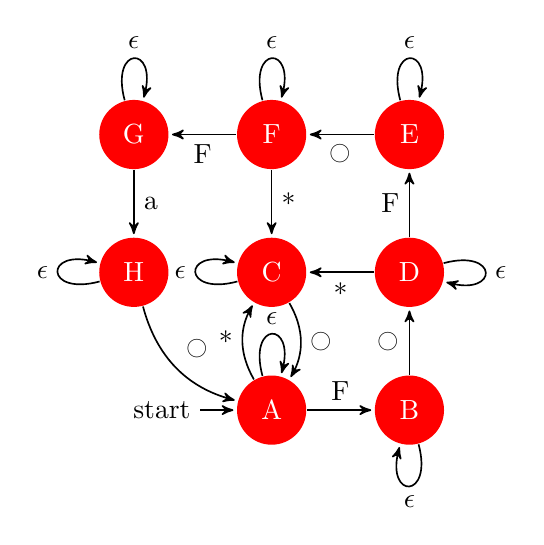
\begin{tikzpicture}[->,>=stealth',shorten >=1pt,auto,node distance=1.75cm,
                    semithick]
  \tikzstyle{every state}=[fill=red,draw=none,text=white]

  \node[initial,state] (A)              {A};
  \node[state]         (B) [right of=A] {B};
  \node[state]         (C) [above of=A] {C};
  \node[state]         (D) [above of=B] {D};
  \node[state]         (E) [above of=D] {E};
  \node[state]         (F) [above of=C]  {F};
  \node[state]         (G) [left of=F, above of=C] {G};
  \node[state]         (H) [below of=G] {H};

  \path (A) edge              node {F} (B)
            edge [loop above] node {$\epsilon$} (A)
            edge [bend left]  node {*} (C)
        (B) edge [loop below] node {$\epsilon$} (B)
            edge              node {$\ocircle$} (D)
        (C) edge [bend left]  node {$\ocircle$} (A)
            edge [loop left] node {$\epsilon$} (C)
        (D) edge [loop right] node {$\epsilon$} (D)
            edge              node {F} (E)
            edge              node {*} (C)
        (E) edge [loop above] node {$\epsilon$} (E)
            edge              node {$\ocircle$} (F)
        (F) edge [loop above] node {$\epsilon$} (F)
            edge              node {F} (G)
            edge              node {*} (C)
        (G) edge [loop above] node {$\epsilon$} (G)
            edge              node {a} (H)
        (H) edge [loop left] node {$\epsilon$} (H)
            edge [bend right]             node {$\ocircle$} (A);
\end{tikzpicture}
\caption{A Monitor State Machine}
\label{fig:state_machine}
\end{figure}

Figure \ref{fig:state_machine} shows the machine corresponding to \code{checkFs}. Each transition is triggered by a clock-tick, the labels on the transitions are: $\epsilon$ when no history is available; \code{F} occurs when the next state element in the history is an \code{F}; $\ocircle$ occurs when there is at least one element at the head of the history and causes the element to be consumed; * denotes the situation when the next state element in the history is anything but \code{F}.

\begin{figure}
\begin{lstlisting}
act nothing {
  Monitor(a,i,s,f) -> 
    s <- Monitor(a,i,self,f)
}

act !(command) {
  Monitor(a,i,s,f) -> {
    command();
    s <- Monitor(a,i,new nothing,f)
  }
}

act p ; q {
  Monitor(a,i,s,f) -> 
    p <- Monitor(a,i,new q + s,f)
}

act p + q {
  Monitor(a,i,s,f) -> 
    p <- Monitor(a,i,s,fun() q <- Monitor(a,i,s,f))
}

box p = new mu(fun(q) new(p ; new circ(box q)))

act circ p { 
  Monitor(a,i,s,f) -> 
    p <- Monitor(a,i+1,s,f) 
}

act ? pred {
  Monitor(a,i,s,f) -> 
    become activate(pred,a,i,s,f)
} 

act activate(pred,actor,i,succ,fail) {
  Monitor(_,_,_,_) -> {};
  Time(_) ->
    if length(actor.history) > i
    then { 
      become ? pred;
      if pred(nth(actor.history,i))
      then succ <- Monitor(actor,i,new nothing,fail)
      else fail()
    } else {}
}

act mu g {
  Monitor(a,c,s,f) -> g(new mu g) <- Monitor(a,c,s,f)
}
\end{lstlisting}
\caption{ESL Monitor Behaviours}
\label{fig:monitor_behaviours}
\end{figure} 

A monitor state machine is implemented as an ESL actor whose behaviour supports two messages. The first message \code{Time(t)} drives the state machine. The second message \code{Monitor(a,c,s,f)} activates the monitor and contains the monitored actor \code{a}, an integer \code{i} that indexes the next element of \code{a.history}, a monitor \code{s} that is used as a {\it success continuation}, and a function \code{f} that is used as a {\it fail continuation}. The key idea is that if \code{m <- Monitor(a,i,s;s',f)} then at some future clock-tick, if \code{m} is able to consume the \code{i}th element from \code{a.history} then \code{s <- Monitor(a,i+1,s',f)} otherwise if \code{m} rejects the \code{i}th element then \code{f()} tries an alternative.

The monitor behaviours are defined in figure \ref{fig:monitor_behaviours}, note that where the clock-tick handler is \code{Time(_) -> \{\}} it is omitted. The simplest monitor has the behaviour \code{nothing} that directly activates the success continuation without modifying any of the supplied data. An action ! is similar to \code{nothing} except that it activates the supplied command. A sequenced monitor \code{p;q} consists of two component monitors \code{p} and \code{q}. When activated, the sequence tries \code{p} adding \code{q} to the success continuation. Alternative \code{p+q} activates \code{p} and adds \code{q} to the fail continuation. The monitor \code{circ p} increments the count \code{i} thereby skipping the next element of the history.

The monitor \code{? pred} changes its behaviour when it is activated in order to check the history of the actor \code{a}. If there is an \code{i}th element in \code{actor.history} then the monitor applies \code{pred} to check whether the indexed history element satisfies the predicate. If so then the successor is activated, otherwise the monitor fails.

Recursive expressions are created using \code{mu g}. An example of recursion is used in the implementation of \code{box} where \code{box p} is unrolled to become \code{p ; circ(p ; circ(p ; circ(p ; ...)))}.

\subsection{Implementation}

\label{sec:implementation}

The specification given in section \ref{sec:specification} defines a sequence of system states that must be refined to produce an ESL simulation model of the system whose levers can be modified and whose goals can be measured. The refinement must produce a system that is consistent with the specification, but that may introduce more detail. The result is an implementation defined in terms of five types of behaviour \code{customer} that models the generation of opportunities, \code{opportunity} that models the bidding and awarding process for opportunities, a notice-board \code{nb}, \code{provider} that models the creation of bids and their outcome, and a monitor for \code{provider} adaptive behaviour. This section gives the key elements of the implementation.

The \code{customer} behaviour is supplied with a colour, a percentage chance of changing the colour, the frequency at which the opportunities are created and the availability of the opportunity:
\begin{lstlisting}[numbers=left]
opp(Red) = Green;
opp(Green) = Red;
act customer(colour,pcChange,frequency,avail) {  
  next = 0;  
  offer()=nb <-Add(new opportunity(self,colour,avail))
  Time(_) when next=frequency -> { 
    next := 0;
    probably(90) {
      offer();
      probably(pcChange) colour := opp(colour) 
    } 
  };        
  Time(_)      ->  { next := next + 1 };
  Done(colour) -> history := history + [colour]           
};
\end{lstlisting}
A customer detects clock-ticks on lines 7 and 14. Every \code{frequency} clock-ticks (line 7) there is a 90\% chance (line 9) that an offer is created (line 10) and a \code{pcChange} chance that the colour changes. A new opportunity is created in line 6 by sending an \code{Add} message to the global notice-board \code{nb}.

An opportunity behaviour is supplied with a customer, the colour of the opportunity and the length of time the opportunity should be available:
\begin{lstlisting}[numbers=left]
act opportunity(customer,colour,available) {
  export customer;
  tryAward(Bid(_,v),true)  = { v <- Failed; true };
  tryAward(Bid(c,v),false) = { v <- Award;  true } 
                             when c = colour;
  tryAward(Bid(_,v),false) = { v <- Failed; false };
  terminate() = {                           
    nb <- Remove(self);                                         
    customer <- Done(colour);
    kill(self)                      
  };
  bids = []                                                     
  b=Bid(colour,vendor) when available > 0 -> 
    bids := b:bids;                       
  Bid(_,vendor)  -> vendor <- Failed;
  Time(_) when (available = 0) and (bids <> []) -> { 
    let won = false 
    in for b in shuffle(bids) do 
         won := tryAward(b,won); 
    terminate()                               
  };
  Time(_) when (available = 0) -> terminate();
  Time(_) -> available := available - 1
};
\end{lstlisting}
An opportunity receives bids from providers (13-15). If the opportunity is available then the bid is saved (14) otherwise the provider has missed the deadline and is informed that the bid has failed (15). Clock-ticks reduce the availability count (23), when the opportunity closes and there are bids (16), the bids are taken in a random order (18) and awarded (3-6). An opportunity is terminated by removing it from the global notice-board (8) and informing the customer that the colour was processed (9). The actor is killed (10) meaning that is can perform no further computation.

A provider is created with a colour that controls the bids:
\begin{lstlisting}[numbers=left]
act provider(colour) {  
  export history;                                                 
  history = [];
  bidding = false;
  record(x) = history := history + [x];
  bid(o:_) = { 
    o <- Bid(getColour(history,o.customer),self); 
    bidding := true 
  };
  getColour([],c) = colour;
  getColour(Changed(c,customer):_,customer) = c;
  getColour(_:h,c) = getColour(h,c)
  Time(_) when (nb.data <> []) and (bidding=false) -> 
    bid(shuffle(nb.data));
  Award -> { record(S); bidding := false };
  Failed -> { record(F); bidding := false };
  Change(customer) -> 
    record(Changed(opp(colour),customer));
  Change(_) -> {};
  Time(_) -> {}
};
\end{lstlisting}
A provider checks the opportunities on the notice-board and makes a bid (13-14,6-9) based on the history (3). A monitor (defined below) adds terms of the form \code{Changed(colour,customer)} to the history of a provider (17,18) which is subsequently used to determine the colour of a bid (10-12) for that customer. The opportunity informs a provider of the outcome of a bid (15,16).

A monitor is created for each provider and customer pair. The predicate \code{hasTail} checks whether the three most recent opportunities produced by a supplied customer are the opposite colour of that for provider bids:
\begin{lstlisting}
change(p,c) = fun() p <- Change(c)
  when hasTail(c.history,three(opp(p.colour)))
  
checkFs(change(p,c)) <- Monitor(p,0,new nothing,fun() {})
\end{lstlisting}
The entire simulation is implemented as an ESL actor with the following behaviour:
\begin{lstlisting}[numbers=right]
act bidding(pc,d,P,C,results,monitors) {
  theirMonitor = head(head(monitors));
  myMonitor    = tail(head(monitors));
  cs = [ new customer(Green,pc,4,4) | c <- 1..C ];
  vs = [ new provider(Red) | v <- 1..P ];
  ms = [ theirMonitor(v,c) | v <- vs, c <- cs ];
  v  = let v = new vendor(Red) 
       in { 
         for c in cs do myMonitor(v,c); 
         v 
       };
  killAll() = {
        for c in cs do kill(c);
        for v in vs do kill(v);
        for m in ms do kill(m);
        kill(v);
  }
  -> print('Start Bidding');
  Time(t) when t = d -> {
    if pc > 5
    then 
      if tail(monitors) = []
      then { stopAll(); print(results) }
      else {
        killAll(v);
        resetTime(0);
        become bidding(0,d,P,C,[],tail(monitors))
      }
    else {
      results := results + [count(S,v.history)];
      killAll();
      resetTime(0);
      become bidding(pc + 1,d,P,C,results,monitors)
    }
  };
  Time(_) -> {}
};
\end{lstlisting}
The behaviour \code{bidding} is supplied with:
\code{pc} the percentage likelihood of each customer changing their colour,\code{d} the duration of the simulation in clock-ticks\code{P} the number of providers other than ourselves, \code{C} the number of customers, \code{results} a list of numbers that represent our successes for each iteration of the simulation, \code{goals} a list of pairs of functions \code{m1:m2} where each function is applied to a vendor and a customer and created a monitor for that vendor with respect to the customer.

A \code{bidding} actor creates \code{C} customers with a \code{pc} chance of changing colour from the initial \code{Green} (line 4). The providers created on line 5 are all of the opposite colour and have monitors created on line 6 for each customer. The vendor that is designated {\it ourselves} is created on lines 7--11 and have a monitor created for each customer.

Each clock-tick the customer, vendor and monitor actors will behave autonomously. The simulation detects when the duration \code{d} has been reached on line 19. The aim is to run the simulation for different values of \code{pc} up to 5 and for different combinations of monitor creation. If the limit has been reached (line 20) then we stop when there are no more monitor combinations to try (line 22). Otherwise, if the limit has been reached and there are outstanding monitor combinations we reset (25--26) and try the rest of the monitors (line 27).
%
If the value of \code{pc} has not reached 5 then the results are extended (line 30), the simulation is reset (lines 31--32) and the simulation is re-run with the next value for \code{pc}.

The bidding behaviour is used to generate results. We need three different types of monitor: {\it none} that does not change a provider, {\it random} that changes a provider's colour at random, and {\it adaptive} that changes a provider's colour based on its failure rate:
\begin{lstlisting}
act random(provider,customer) {
  Time(_) -> {
    colour := opp(colour); 
    vendor <- Change(customer) 
  }
};
\end{lstlisting}
The monitors will be created dynamically in the simulation so appropriate functions are created that can be called as required:
\begin{lstlisting}
randomMonitor(p,c)   = new random(p,c);
noMonitor(p,c)       = new inoperable;
adaptiveMonitor(p,c) = 
  checkFs(change(p,c)) <- Monitor(p,0,new nothing,fun() {})
monitors = [randomMonitor,noMonitor,adaptiveMonitor];
\end{lstlisting}
Finally, an ESL program must define a behaviour called \code{main} that has the same function as the class called \code{Main} in Java. The bidding simulation is to be run for \code{1000} clock-ticks with \code{10} providers and \code{2} customers:
\begin{lstlisting}
act main {
  -> new bidding(0,1000,10,2,[], me * them);
  Time(_) -> {}
}
\end{lstlisting}

\subsection{Results}

\label{sec:results}
Figure \ref{fig:results} shows the results of the simulation given 2 customers and two categories of service provider: {\it competitors} (10) and {\it ourselves} (1). Each category of service provider can have three different adaptor types:
\begin{description}
\item[none] No adaptive behaviour: the provider will not change the colour of the bid.
\item[random] The provider changes its bid colour at random.
\item[adaptive] The provider uses a monitor on all customer histories in order to change bid colour when it has failed to be awarded an opportunity 3 or more times.
\end{description}
The simulation was executed for 1000 clock-ticks for each configuration of service service provider category and adaptor type. The number of successful bids for ourselves and the maximum number of successful bids for competitors was recorded for each configuration. 
%
\begin{figure}[t]
\centering
\includegraphics[width=\columnwidth]{sample}
\caption{Results}
\label{fig:results}
\end{figure}
%
%
Figure \ref{fig:results} shows results for a selection of configurations: the legend labels each result line in terms of configuration strategies ({\it ourselves}, {\it competitors}) and shows the number of successes for ourselves. 

The simulation is intended to aid decision making with respect to whether a particular strategy is cost effective, and although we would need to know the cost of monitoring historical records, the results indicate that it is clearly in our favour to implement the adaptive strategy if we believe that our competitors are behaving randomly. Also, it would appear that no strategy at all is of similar value to random choice. Where all categories are behaving strategically, there is a benefit to us, however this is significantly less that when our competitors are not strategic.

\section{Evaluation}

\label{sec:evaluation}

Section \ref{sec:bidding} has described a synthetic case study used to demonstrate a simulation-based approach to decision-making in terms of the conceptual model given in section \ref{sec:concepts} and the ESL language in \ref{sec:implementation}. We have used the approach on a real-world industrial business processing outsourcing (BPO) case study as described in this section.

\begin{figure}[t]
\centering
\includegraphics[width=0.75\columnwidth]{sm}
\caption{BPO State Machine}
\label{fig:BPO_state_machine}
\end{figure}

An outsourcing deal starts with a customer RFP inviting bids for a business process. An interested service provider's bid includes the number of full time employees (FTEs) to be deployed and billing rate (BR), its {\it capability ranking} (CR) via an independent agency, track record, any particular strengths such as number of capable employees, domain knowledge, {\it etc}. At the end of the bidding phase the customer evaluates all bids and identifies a service provider for outsourcing. Soft issues such as familiarity with the processes being outsourced, rapport with the service provider {\it etc.}, also play a part in selection. It is common observation that BPO contracts come up for renewal after 3-5 years where the contract may be renewed on modified terms (typically advantageous to the customer) or may go for rebidding. The factors that influence renewal include rate reductions, number and degree of escalations, quality perceptions. Figure \ref{fig:BPO_state_machine} shows a representative state transition diagram of BPO business.

The BPO environment is modelled as a set of customer (C) units, business processes (BP) units and service provider (SP) units. The goals of customer units are to save costs and improve effectiveness; the goals of service provider units are to increase revenue, realisation ({\it i.e.}, revenue per FTE per hour) and size in terms of FTE numbers; the goals of business process units is to optimise its operational cost.
%
All units encapsulate their characteristics as data. For example, service providers have data representing CR, BR, FTE count, market influence and delivery excellence expressed as a fixed value, a range of values or a probabilistic distribution. For example, CR is one of: {\it contender}, {\it challenger}, {\it visionary}, or {\it  leader}, BR is a range ({\it e.g.}, \$8  to \$10 per hour per FTE) and quality is a probability distribution describing confidence of delivering {\it excellent}, {\it normal} and {\it below normal} services. 

BPO events have a certain frequency and are stochastic in nature. When the customer raises an RFP, all interested service providers respond by selecting values from their characteristics variables. The bid evaluation function is a weighted aggregate of the various elements of RFP response and a random value to capture effect of inherent uncertainty. The service provider with the lowest computed value of a bid wins the outsourcing deal which gets executed by selected service provider. The decision to renew existing contract is modelled on similar lines. New processes may emerge as candidates for outsourcing are no longer needed. The existence of customers and service providers may also change with the time.
 
Units observe the visible history of other actors while reacting to an event and try to adapt if its goals are not achievable. The service providers are equipped with two negotiation levers: FTE productivity and billing rate. A BPO service provider must make decisions that address market share, internal growth, {\it etc.} In the interest of space we focus on question: With the current strategy how much market share will a provider capture and how much revenue opportunity will be lost? Other service providers are considered as competitors and the modelled provider will be referred to as SP. 

\begin{figure}
\includegraphics[width=\columnwidth]{fte}
\caption{BPO Goal Measurement}
\label{fig:BPO_goals}
\end{figure}

\begin{figure}
\includegraphics[width=\columnwidth]{img}
\caption{BPO Revenue Share}
\label{fig:BPO_revenue_share}
\end{figure}
%The case study was represented using ESL and simulated for 10 years with goals for revenue, FTE numbers and realisation shown in blue, green and dotted red in figure \ref{fig:BPO_goals}. The SP revenue share is shown in figure \ref{fig:BPO_revenue_share} where the current SP revenue is 446.5 M USD with a 60\% unexplored market where grey represents the revenue of the competitors and white at the bottom of the bar indicates the SP revenue loss. SP revenue increases, the number of deployed FTEs is increases, but SP realisation factor decreases to an extent as shown using in blue, green and red lines in figure \ref{fig:BPO_goals}. After 10 years the total revenue increases from 620 M USD to 1165 M USED, the SP revenue increases from 446.54 M USD to 922.28 M USD but market share is reduced from 40\% to 34\% of total revenue (figure \ref{fig:BPO_revenue_share}). The graph in figure \ref{fig:BPO_revenue_share} also indicates a little revenue loss due to the loss in renewal process. 

The case study was represented using ESL and simulated for 10 years with goals for revenue, FTE numbers and realisation shown in blue, green and dotted red in figure \ref{fig:BPO_goals}. The SP revenue share is 
shown in figure \ref{fig:BPO_revenue_share} where the current SP revenue is \$441.66M  with a 60\% unexplored market where grey represents the revenue of the competitors and white at the bottom of the bar indicates the SP 
revenue loss. SP revenue increases, the number of deployed FTEs is increases, but SP realisation factor decreases from 14.9 to 14.3  as shown using in blue, green and red lines in figure \ref{fig:BPO_goals}. After 10 years the 
total revenue increases from \$1115.88M to \$2571.44M, the SP revenue increases from \$441.66M to \$922.28M but market share is reduced from 40\% to 35\% of total revenue (figure \ref{fig:BPO_revenue_share}). The graph in figure \ref{fig:BPO_revenue_share} also indicates a little revenue loss due to the loss in renewal process.

The graphs indicate many interesting aspects about SP: it is negotiating well for deal renewal, however there is a significant scope for improving revenue share for FTE and FTE realisation. This could be improved by winning more deals and by increasing the billing rate. However, winning more deals without compromising the billing rate is hard problem. The options such as increasing productivity with better resources and market influence should be exploited for an optimum solution and the ESL-based simulation can be used to explore the options.


\section{Conclusion}

\label{sec:conclusion}

This paper has defined an approach that aims to support organisational decision-making in terms of a conceptualisation of the key features and a technology platform. The approach is based on a computational view of an organisation that is encoded using actors. We have used a simple bidding scenario to demonstrate the features, including adaptive behaviour, and have described a real-world case study that has produced results that could be used to support management decisions. 

All the code in the paper has been implemented in the ESL language which runs on a VM written in Java and which we claim is a suitable basis for building abstractions for organisational simulation including ideas from multi-agent systems including collaboration and negotiation. 

Further work is planned in the following areas: ESL currently lacks a static type system which will help to engineer large-scale simulations. Although we have identified an approach to specification of a simulation given in section \ref{sec:specification}, no attempt has been made to verify properties of the ESL program; research in this area \cite{yasutake2015actario} will be investigated. ESL has been designed with the aim of expressing patterns of organisational behaviour, and with the expectation that results from Multi-Agent Systems research will be relevant to constructing organisational simulation models. We intend to investigate how to encode features such as negotiation and collaboration. 

\clearpage

\bibliographystyle{abbrvnat}
\bibliography{bib}

\end{document}


